\documentclass[UTF8,a4paper,cs4size,hyperref]{ctexart}

\title{毕业设计论文草稿}
%\begin{large}\qquad \qquad \qquad—— \end{large}}
\author{姓名:张雪悦\ \ 班级:微32\ \ 学号:2013011756}
%\date{\today}

\usepackage[left=31.75mm,right=31.75mm]{geometry}
\usepackage{upgreek}
\usepackage{hyperref}
\usepackage{booktabs}
\usepackage{tabularx}
\usepackage{graphicx}
\usepackage{amsmath}



\hypersetup{
colorlinks=false}



\pagestyle{plain}

\bibliographystyle{unsrt}

\begin{document}

\maketitle

\section{二氧化硅微型谐振腔的二次谐波产生}
\subsection{理论基础}
\subsubsection{基于电偶极子的二次非线性}
\label{sec:dipole}
在经典光学中,介质与电磁波的相互作用通常用介质极化率来描述,这一介质极化率随电场变化的函数关系可以展开为电场的幂级数,
\begin{equation}
P(t) = \epsilon_0(\chi^{(1)}E(t)+\chi^{(2)}E^2(t)+\chi^{(3)}E^3(t)+\dots)
\end{equation}
线性项被归入介质折射率中,而一阶以上的项就进入了非线性光学的范畴。非线性极化率又可以作为波动方程中的源激发出新的辐射场。
\begin{equation}
\nabla^2E-\frac{n^2}{c^2}\frac{\partial^2E}{\partial t^2} = \frac{1}{\epsilon_0c^2}\frac{\partial^2P^{NL}}{\partial t^2}
\label{eq:wave}
\end{equation}
不同阶数的非线性项将引出不同的非线性过程,这里我们主要着眼于二阶非线性项,即与$\chi^{(2)}$有关的项。

首先考虑单一频率的光输入,
\begin{equation}
E(t) = E_0e^{-i\omega t}+\textrm{c.c.} 
\end{equation}
	其中c.c.表示复共轭。这样的输入在具有二次非线性的材料当中将激发出如下的极化率
\begin{equation}
P^{(2)}(t) = 2\epsilon_0\chi^{(2)}E_0E_0^*+(\epsilon_0\chi^{(2)}E_0^2e^{-2i\omega t}+\textrm{c.c.})
\end{equation}
可以看到第一项对应着一个直流分量,不激发辐射场,被称作光学整流效应optical rectification。而第二项就产生了新的频率分量,从量子光学的角度来看,可以看成是材料中的原子吸收了两个光子,又产生了一个能量等于两个光子之和的二倍频光子,如图\ref{pic:energyLevel}(a)。

\begin{figure}
\centering
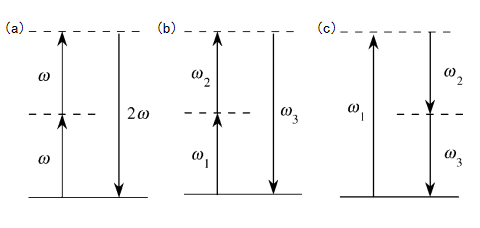
\includegraphics[scale=0.8 ]{energyLevel.png}
\caption{二次非线性过程的能级示意图。(a)二次谐波产生。(b)二次合频信号产生。(c)二次差频信号产生。图引自\cite{boyd2003nonlinear}}
\label{pic:energyLevel}
\end{figure}

当我们考虑输入光由两种频率组成,则可以通过二阶非线性产生合频和差频效应。电场可以写成
\begin{equation}
E(t) = E_1(t)e^{-i\omega_1 t}+E_2(t)e^{-i\omega_2 t}+\textrm{c.c.}
\end{equation}
该电场通过具有二次非线性的材料之后,将产生具有若干不同频率分量的极化率$P^{(2)}(t) = \sum_n P(\omega_n)e^{-i\omega_nt}$,包括
\begin{gather}
P(2\omega_1) = \epsilon_0\chi^{(2)}E_1^2 \ \ \textrm{(SHG)} \notag \\
P(2\omega_2) = \epsilon_0\chi^{(2)}E_2^2\ \  \textrm{(SHG)} \notag \\
P(\omega_1+\omega_2) = \epsilon_0\chi^{(2)}E_1E_2\ \  \textrm{(SFG)}  \\
P(\omega_1-\omega_2) = \epsilon_0\chi^{(2)}E_1E_2^*\ \  \textrm{(DFG)} \notag \\
P(0) = \epsilon_0\chi^{(2)}(E_1E_1^*+E_2E_2^*)\ \  \textrm{(OR)} \notag 
\end{gather}
其中SHG代表二次谐波产生,SFG代表二次合频信号产生,可以由图\ref{pic:energyLevel}(b)的过程来表示,DFG则是差频信号产生,可以由图\ref{pic:energyLevel}(c)的过程来表示。

介质的介电常数$\epsilon_0\chi$和材料的性质紧密相关,在经典理论当中,可以将材料中的原子(原子核+电子)看成是一个谐振子,标准的抛物线型谐振子势会带来材料的线性响应,而偏离抛物线型的谐振子势则是非线性响应的源头。

在非标准抛物线势中,又可以分为两种,一种是具有中心对称性的势,另一种是不具有中心对称性的势,一维的情况如图\ref{pic:potential}所示。电子的运动方程可以写成
\begin{equation}
\ddot{x}+2\gamma\dot{x}+\omega_0^2x+ax^2+bx^3 = -eE(t)/m
\end{equation}
其中左边第二项是阻尼项,后面的三项是谐振子势带来的加速度,右边是外加电场对于电子的影响。由此方程,结合微扰法,可以推出使用这种模型近似下的$\chi$与谐振子势的非线性系数$a$, $b$的关系\cite{boyd2003nonlinear}。其中,二次非线性系数$\chi^{(2)}$与谐振子的非对称势系数$a$成正比,即,如果材料具有中心对称性($a=0$),或材料是非晶态的(各个方向的非对称响应抵消),则$\chi^{(2)}=0$。

也可以从更高的层面上理解这个结论,对于二次谐波对应的极化率
\begin{equation}
P(t) = \epsilon_0\chi^{(2)}E^2(t),
\end{equation}
如果将电场反向,即上式中的$E(t)$变为$-E(t)$,由式子本身来看极化率不变,而根据中心对称性或非晶态材料性质,电场反向的时候,极化率也应当反向。由此推出在这类材料当中的二阶非线性极化率始终为0.

\begin{figure}
\centering
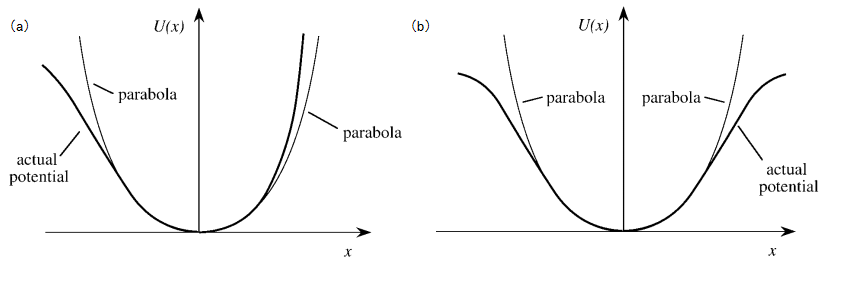
\includegraphics[scale=0.6 ]{potential.png}
\caption{原子的一维非标准抛物线势。(a)非中心对称势。(b)中心对称势。图引自\cite{boyd2003nonlinear}}
\label{pic:potential}
\end{figure}

从\ref{pic:response}中可以更加直观地看到,中心对称材料或非晶态材料的极化率随电场的变化虽然比起标准正弦形式有所变形,但依然是奇函数,不含偶次分量,即没有二次非线性响应,而非中心对称材料则会呈现出含偶次分量的特点。

\begin{figure}
\centering
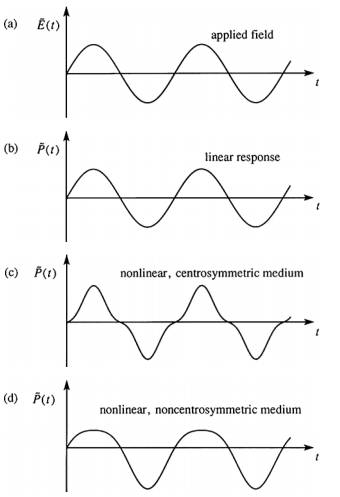
\includegraphics[scale=1 ]{response.png}
\caption{不同材料的极化率响应。图引自\cite{boyd2003nonlinear}}
\label{pic:response}
\end{figure}

\subsubsection{在介质表面或界面处的二次非线性}
虽然中心对称或非晶态材料的体内缺乏偶极近似下的二次非线性,在介质表面处,这种对称性被破坏,例如,最外层的原子向介质两侧振动所感受到的势是不一致的,这就会导致二次非线性的产生,同时,从直观上来看,只有靠近表面的一个薄层内具有这种表面非线性。

这里,我们在理论上探究一种最简单的情况,界面是平面,两种波长的光入射,两侧介质均为中心对称介质。将具有非线性的一个薄层抽象出一个单独的介电常数,并使其厚度趋近于0。原理图如图\ref{pic:surface},这里考虑两束光($\omega_1$, $\omega_2$)以不同的入射角射在材料界面出同一位置,反射波和投射波中都带有了新的频率分量。考虑非线性极化率的麦克斯韦方程组为
\begin{gather}
\nabla \cdot \mathbf{D}  = -\nabla \cdot \mathbf{P^{nls}} , \\
\nabla \times \mathbf{E }	+ \frac{\partial\mathbf{B} }{\partial t} = 0, \\
\nabla \cdot \mathbf{B} = 0, \\
\nabla \times \mathbf{H} - \frac{\partial \mathbf{D}}{\partial t} = \frac{\partial \mathbf{P^{nls}}}{\partial t}.
\end{gather}
由这一组方程组,结合界面两侧的边界条件,可以推出\cite{heinz1991second}
\begin{gather}
\Delta D_z = -\nabla_t \cdot \mathbf{P_s^{nls}}, \\
\Delta E_t = -1/\epsilon' \nabla_t P_{s,z}^{nls}, \\
\Delta B_z = 0, \\
\Delta \mathbf{H_t} = \partial \mathbf{P_s^{nls}}/\partial t \times \mathbf{\hat z} 
\end{gather}
其中$\Delta X = X(0^+)-X(0^-)$, $\mathbf{P^{nls}}  = \mathbf{P_s^{nls}}\delta(z)$,$\epsilon'$是界面层中的介电常数。通过上述表达式,借助菲涅耳修正,可以最终推出由这一层非线性极化层带来的向两种介质中辐射的电场信息\cite{heinz1991second}。
\begin{figure}
\centering
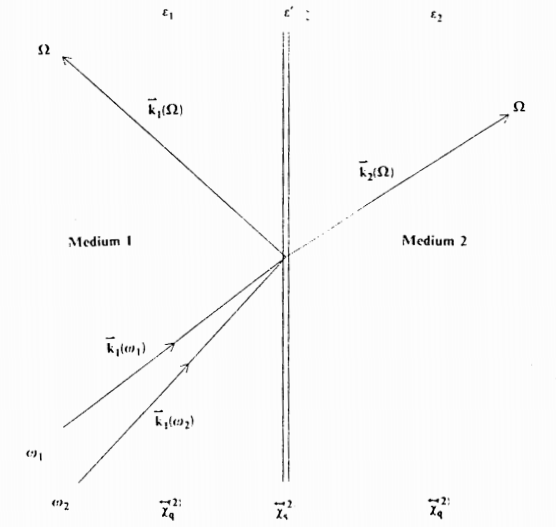
\includegraphics[scale=1 ]{surface.png}
\caption{界面二次非线性示意图。图引自\cite{heinz1991second}}
\label{pic:surface}
\end{figure}

在微型谐振腔中,依然可以通过考虑表面的非线性极化层来解决问题。具体有两种方式,一种将极化层看成厚度无限小的薄层,另一种则直接将极化层处理为空间上的$\delta$函数。首先来看第一种方法,设基波、二次谐波的电场为
\begin{equation}
\mathbf{E}_i(x,y,z,t) = a_i(t)\mathbf{E}_{0i} (x,y,z)e^{-i\omega_it},
\end{equation}
其中$i = 1, 2$分别代表基波和二次谐波,$\mathbf{E}_{0i} (x,y,z)$是空间腔膜分布,$a_i(t)$是慢变电场幅值,$\omega_i$是光场频率。由式\ref{eq:wave},得
\begin{equation}
a_2(t)\nabla^2\mathbf{E}_{02}e^{-i\omega_2t}-\frac{n^2}{c^2}\frac{\partial^2a_2(t)e^{-i\omega_2t}}{\partial t^2}\mathbf{E}_{02} = \frac{1}{\epsilon_0c^2}\frac{\partial^2\mathbf{P}^{NL}}{\partial t^2},
\end{equation}
其中
\begin{equation}
\mathbf{P}^{NL} = a_1^2(t)e^{-2i\omega_1t}\chi^{(2)}:\mathbf{E}_{01}\mathbf{E}_{01}
\end{equation}
由于$d^2 a_2/d t^2 << -i\omega_2\cdot d a_2/d t $,只保留后一项,同时注意到由于$\mathbf{E}_{02}$是腔膜的空间分布,在线性情况下满足普通波动方程
\begin{equation}
\nabla^2\mathbf{E}_{02}e^{-i\omega_2t}-\frac{n^2}{c^2}\frac{\partial^2e^{-i\omega_2t}}{\partial t^2}\mathbf{E}_{02} = 0 
\end{equation}
故由二阶非线性极化层带来的二次谐波幅度增速为
\begin{equation}
\frac{da_2}{dt} = g_sa_1^2e^{-i(2\omega_1-\omega_2)t},
\end{equation}
其中
\begin{equation}
g_s = 2i\frac{\omega_1^2}{\omega_2n^2}\frac{\int \mathbf{E}_{02}^*:\chi^{(2)}_s:\mathbf{E}_{01}\mathbf{E}_{01} d\mathbf{V}}{\int |\mathbf{E}_{02}|^2 d\mathbf{V}}
\end{equation}
注意$\chi^{(2)}$只在表面附近的区域内不为0,如果采用表面非线性系数,则分子上的积分化为$\int \mathbf{E}_{02}^*:\chi_s^{(2)}:\mathbf{E}_{01}\mathbf{E}_{01} d\mathbf{S}$。

考虑实际的腔膜还有耗散,输入输出,失谐等关系,可以得出基波、二次谐波腔膜幅度的耦合模方程\cite{haus1991coupled}
\begin{gather}
\label{eq:cpmode}
\frac{da_1}{dt} = -(\frac{\kappa_{10}+\kappa_{1e}}{2} )a_1+\sqrt{\kappa_{1e}}se^{-i(\omega_s-\omega_1)t}+g_s^*a_1a_2^*e^{i(2\omega_1-\omega_2)t} \\
\frac{da_2}{dt} = -(\frac{\kappa_{20}+\kappa_{2e}}{2})a_2+g_sa_1^2e^{-i(2\omega_1-\omega_2)t}
\end{gather}
其中$\omega_i$为腔膜的频率,$s$为输入驱动,$|s|^2$是输入功率,$\omega_s$是输入光频率,$\kappa_i0, \kappa_ie$分别是内在损耗和耦合损耗,与光学品质因子$Q$之间的关系为$\kappa_i = \omega_i/Q_i$。

将表面非线性层处理为$\delta$函数的方法比较繁琐,可参看\cite{kozyreff2008whispering}。

\subsubsection{由体多极效应带来的二阶非线性}
在\ref{sec:dipole}中计算的二阶非线性都是在电偶极子近似下进行的,在这种情况下,中心对称或非晶态材料中不存在二阶非线性。然而,当我们考虑更高阶的效应,如电四极子和磁偶极子时,在这些材料中依然可以出现二阶非线性。

体多极效应带来的二阶非线性可以由自由能量密度来计算\cite{bloembergen1965nonlinear,shen1984principles},化简之后的体多极效应可以表示为
\begin{equation}
P^{NL}_i = \gamma\nabla_i(\mathbf{E}\cdot\mathbf{E})+(\delta-\beta-2\gamma)(\mathbf{E}\cdot\nabla)E_i+\beta(\nabla \cdot \mathbf{E})E_i+\zeta E_i\nabla_iE_i
\label{eq:surfaceN}
\end{equation}
其中$\gamma, \delta, \beta, \zeta$是用来描述体效应的系数。其中第三项在均匀体介质中,由于$\nabla \cdot \mathbf{E}=0$所以不存在,而在非晶态材料(如熔融二氧化硅)中,$\zeta=0$,第四项也为0。可以看到,第一项对应着一个纵波$\mathbf{P}_\gamma =  \gamma\nabla(\mathbf{E}\cdot\mathbf{E})$,即,$\nabla \times \mathbf{P}_\gamma = 0$,这样的源在均匀介质当中是不会激发出辐射场的(磁场分量始终为0),然而当这个纵波传播到介质界面处的时候,则可以耦合产生正常的电磁波,并且根据边界条件计算,无论对于怎样的场分布,这一项对二次谐波产生带来的贡献将与上一节所述的表面二次非线性不可区分\cite{sipe1987new},由这一项带来的等效表面非线性系数可以写成\cite{heinz1991second}
\begin{gather}
(\chi^{(2)}_{s,\gamma})_{\perp \parallel \parallel} = \gamma_1\frac{\epsilon '(\Omega)}{\epsilon_1(\Omega)}-\gamma_2\frac{\epsilon '(\Omega)}{\epsilon_2(\Omega)}, \\
(\chi^{(2)}_{s,\gamma})_{\perp \perp \perp} = \gamma_1\frac{\epsilon '(\Omega)}{\epsilon_1(\Omega)}(\frac{\epsilon '(\omega)}{\epsilon_1(\omega)})^2-\gamma_2\frac{\epsilon '(\Omega)}{\epsilon_2(\Omega)}(\frac{\epsilon '(\omega)}{\epsilon_2(\omega)})^2
\end{gather}
其中$\epsilon ', \epsilon_1$和$\epsilon_2$分别是表面层,界面两侧的介电常数,$\Omega, \omega$分别是二次谐波和基波的频率。

在同一材料体系中,在实验上除非能够测量体内纵波的情况,否则不能通过改变光场分布来对这两种效应加以区分。另一种更具有可行性的方法则是,换用不同体和界面参数的材料进行实验,然后推知此项效应。

总而言之,式\ref{eq:surfaceN}中第一项与表面非线性无法区分,第二项是体效应,可以通过变换不同的光场分布测得材料的响应系数,第三、四项对于熔融二氧化硅来说为0.

在微型谐振腔中,第一项的贡献可以与表面非线性和在一起,写成一个等效的表面非线性系数
\begin{equation}
g_s = 2i\frac{\omega_1^2}{\omega_2n^2}\frac{\int \mathbf{E}_{02}^*:(\chi^{(2)}_s+\chi^{(2)}_{s,\gamma}):\mathbf{E}_{01}\mathbf{E}_{01} d\mathbf{S}}{\int |\mathbf{E}_{02}|^2 d\mathbf{V}}
\label{eq:gs}
\end{equation}


第二项的贡献可以写成另一个等效的基波、二次谐波耦合系数
\begin{equation}
g_b =  2i\frac{\omega_1^2}{\omega_2n^2}\frac{\int \mathbf{E}_{02}^* \cdot (\delta-\beta-2\gamma)(\mathbf{E}_{01}\cdot\nabla)\mathbf{E}_{01} d\mathbf{V}}{\int |\mathbf{E}_{02}|^2 d\mathbf{V}}
\label{eq:gb}
\end{equation}

最终的耦合模方程可以写为
\begin{gather}
\label{eq:cpmode}
\frac{da_1}{dt} = -(\frac{\kappa_{10}+\kappa_{1e}}{2})a_1+\sqrt{\kappa_{1e}}se^{-i(\omega_s-\omega_1)t}+(g_s+g_b)^*a_1a_2^*e^{i(2\omega_1-\omega_2)t} \\
\frac{da_2}{dt} = -(\frac{\kappa_{20}+\kappa_{2e}}{2})a_2+(g_s+g_b)a_1^2e^{-i(2\omega_1-\omega_2)t}
\label{eq:cpmode2}
\end{gather}

由于通过实验无法直接测量$g_s$中来自表面项和$\gamma$项的相对大小,通过理论估计,利用\cite{terhune1987second}中的数据计算,得$\chi^{(2)}_s/\chi^{(2)}_{s,\gamma}\approx 6.2$。$g_s$与$g_b$的比较可以利用\cite{rodriguez2008calibration}中给出的实验数据,但是具体数值大小依赖于基波模式和二次谐波模式的空间分布,以直径为62$\mu m$的球腔中基波模式为TM偏振,径向量子数$q$为1,角向$l$和方位角向量子数$m$均为171的模式(基模),二次谐波为TM偏振,径向量子数$Q$为2(出于相位匹配的考虑,见下一节),角向$L$和方位角向量子数$M$均为342的模式为例,得到$|g_b|/|g_s|\approx12.09$。

对于球腔来说,偏振方向以$\mathbf{r}\cdot\mathbf{H} = 0$为TM方向,$\mathbf{r}\cdot\mathbf{E} = 0$为TE方向。径向、角向和方位角向量子数的示意见图\ref{pic:mode}
\begin{figure}
\centering
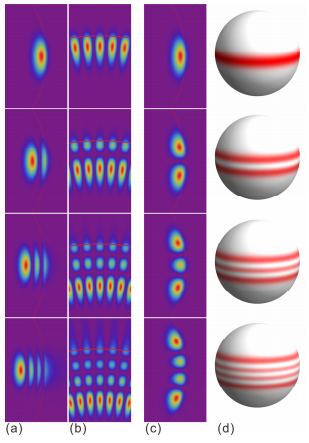
\includegraphics[scale=1 ]{mode.png}
\caption{一些不同模式数的回音壁模式的场分布。(a), 上到下依次为方位角向量子数 = 50, 径向量子数= 1\~4的模式在截面上的场分布。 (b),从上到下依次为方位角向量子数 = 50, 径向量子数 = 1\~4的模式在赤道面上的场分布。 (c),从上到下依次为径向量子数 = 1, 方位角向量子数 = 50, 49,48, 47的模式在截面上的场分布。 (d),从上到下依次为模式数为径向量子数 = 1, 方位角向量子数 = 50, 49, 48, 47的模式在微球表面上的场分布。图引自\cite{LiBeiBei2014}}
\label{pic:mode}
\end{figure}

\subsubsection{空间交叠积分及双共振条件}
\label{sec:2Resonance}
式\ref{eq:gs} \ref{eq:gb}的耦合系数表达式中均含有空间交叠积分,其中$g_s$的空间积分在球坐标系下对应着量子力学中的CG系数,即,需要$M=2m$, $0\le L \le 2l$,这时$g_s$才不为0。对于$g_b$,因为还涉及空间微分,所以还需考虑空间分布函数的奇偶性。总而言之,两模式之间是否有非线性耦合,不仅与材料是否有较大的非线性系数有关,还与空间交叠积分是否不为0有关。

将式\ref{eq:cpmode}\ref{eq:cpmode2}中的$a_1, a_2$换到旋转坐标系中来求解耦合模方程,$\tilde{a}_1 = a_1e^{i(\omega_s-\omega_1)t}$, $\tilde{a}_2 = a_2e^{i(2\omega_s-\omega_2)t}$,做这样变换后的耦合模方程可以写成
\begin{gather}
\label{eq:cpmoder}
\frac{d\tilde{a}_1}{dt} = [i(\omega_s-\omega_1)-\frac{\kappa_{20}+\kappa_{1e}}{2}]\tilde{a}_1+\sqrt{\kappa_{1e}}s+(g_s+g_b)^*\tilde{a}_1\tilde{a}_2^* \\
\frac{d\tilde{a}_2}{dt} = [i(2\omega_s-\omega_2)-\frac{\kappa_{20}+\kappa_{2e}}{2}]\tilde{a}_2+(g_s+g_b)\tilde{a}_1^2
\label{eq:cpmoder2}
\end{gather}

在稳态情况下,假设二次谐波产生对基波的幅度不产生影响(在二次非线性极弱的介质,如二氧化硅中是成立的),上面两式可推出输出的二次谐波功率和输入基波功率之间的关系
\begin{equation}
P_2 = \kappa_{2e}\frac{|g_s+g_b|^2}{(2\omega_s-\omega_2)^2+(\frac{\kappa_{20}+\kappa_{2e}}{2})^2}\frac{\kappa_{1e}P_1^2}{(\omega_s-\omega_1)^2+(\frac{\kappa_{10}+\kappa_{1e}}{2})^2}
\end{equation}
可以看到,在损耗和非线性耦合一定的情况下,输入光与腔膜之间的失谐越小,二次谐波的功率就越大。并且,我们希望输入光与基波、二次谐波同时达到共振,这需要满足$\Delta \omega = \omega_2 - 2\omega_1=0$,即双共振条件。

在晶体非线性光学当中,由于光频是连续分布的,故需要满足的是两种频率具有尽量接近的波矢$k$,即通常所说的相位匹配条件。而在微型谐振腔中,相位匹配条件由角量子数关系$M=2m$来满足,但同时,由于腔膜频率是分立的,因而还需要满足双共振条件来确保二次谐波的有效产生。

由于微型谐振腔中存在色散,包括材料色散和几何色散,色散使得腔中满足相位匹配条件的两个基模模式并不能满足双共振条件,图\ref{pic:mode}(a)就展示了在直径为60$\mu m$的二氧化硅微球腔中的二次谐波(SH)与基波(FW)的色散情况。可以看到,由于不同径向量子数的模式色散情况不一致,事实上可以选用SH与FW拥有不同径向量子数的情况来实现双共振条件。如,图中所示选取FW的q=1,SH的q=2,在角向量子数$l=166$附近可以实现较好的双共振条件。然而需要指出的是,即使使用这样的方法,也不能够保证精确的双共振。首先,由于模式的分立性(即,色散曲线上实际是一个个单独的点),虽然在$l=166$附近的曲线一定具有双共振,但这里并不一定有模式,如图\ref{pic:mode}(b)中的红色点所示,在这种条件下效率最好的模式由于双共振条件带来的功率降低也在$10^{-6}$量级,并且随着模式数的变化,效率也急剧下降。另一方面,实验中很难精确控制球腔的几何形状,比如直径或球的非理想性等等,以直径变化为例,图\ref{pic:mode}(b)中三种不同的直径相差极小,但是对双共振条件带来的效率影响极大,在同一波长范围内,直径稍微变动就会使得效率急剧下降。

\begin{figure}
\centering
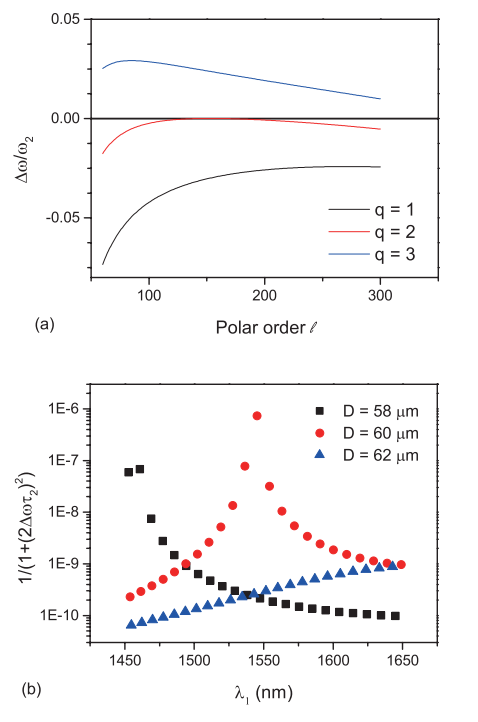
\includegraphics[width=11cm]{disp_ed2_ai.png}
\caption{\textbf{Frequency mismatch induced by dispersion. a,}   Calculated relative
frequency mismatch between SH with different radial orders q and FW as a function of
the polar order of FW.   \textbf{b,}  The calculated off-resonance coefficient of the
q = 2 mode family in microspheres with different diameters D versus the wavelength of
FW. The symbols represent modes with different polar orders separated by a free spectra
range of around 10nm.}
\label{pic:mode}
\end{figure}

为了能在实验中观察到二次谐波,必须采取其他方法来实现双共振。在上述分析当中,没有考虑微型谐振腔的热效应和Kerr非线性。这两种效应都会使得腔膜频率随着输入光功率的变化而发生变化,从而给实现双共振条件提供了可能。

在微腔中起作用的热效应主要包括热折变和热膨胀,热折变是指材料温度发生变化后,折射率也随之发生变化;而热膨胀指的是腔的体积随着温度发生变化。这两种效应结合起来,将使得腔中模式的频率发生变化,对于二氧化硅来说,单位温度变化带来的相对腔膜波长变化为$6\times 10^{-6} K^{-1}$\cite{nikogosyan2003properties,carmon2004dynamical}。较为完整的腔中热过程模型应当理解为,腔膜处能量增加,温度升高,且此热量向腔中非腔膜处及腔外扩散\cite{ilchenko1992thermal},最终达到热平衡,在新的温度下考虑此时的腔膜频率。

而Kerr效应则来源于三阶非线性系数$\chi^{(3)}$,介质极化率除了线性分量还有一个三阶非线性分量也可以产生同样频率的电磁波,$P(\omega) = \epsilon_0(\chi^{(1)}+\chi^{(3)}E(\omega)E(\omega)^*)E(\omega)$,因此也同样会产生一个随着腔中能量变化的折射率,进而引起腔膜频率的变化。

考虑这两种效果之后,得到新的耦合模方程,同样认为二次谐波的能量远远小于基波的能量,因而忽略二次谐波带来的热效应。
\begin{gather}
\label{eq:cpmodec}
\frac{d\tilde{a}_1}{dt} = [i(\omega_s-\omega_1)+iB_{11}|\tilde{a}_1|^2-\frac{\kappa_{20}+\kappa_{1e}}{2}]\tilde{a}_1+\sqrt{\kappa_{1e}}s+(g_s+g_b)^*\tilde{a}_1\tilde{a}_2^* \\
\frac{d\tilde{a}_2}{dt} = [i(2\omega_s-\omega_2)+iB_{12}|\tilde{a}_1|^2-\frac{\kappa_{20}+\kappa_{2e}}{2}]\tilde{a}_2+(g_s+g_b)\tilde{a}_1^2
\label{eq:cpmodec2}
\end{gather}
其中,
\begin{gather}
B_{11} = \frac{\int|\mathbf{E}_{01}|^4d\mathbf{V}}{\int|\mathbf{E}_{01}|^2d\mathbf{V}}[\frac{3\chi_{Kerr}\omega_1}{n_1^2}+(\frac{\partial n}{\partial T})_{eff}\frac{\epsilon_0}{\rho C \delta_{\theta 1}}\frac{\omega_1^2}{Q_{1,abs}}], \\
B_{12} = \frac{\int|\mathbf{E}_{01}|^2|\mathbf{E}_{02}|^2d\mathbf{V}}{\int|\mathbf{E}_{02}|^2d\mathbf{V}}[\frac{6\chi_{Kerr}\omega_2}{n_2^2}+(\frac{\partial n}{\partial T})_{eff}\frac{\epsilon_0}{\rho C \delta_{\theta 2}}\frac{\omega_1\omega_2n_1^2}{n_2Q_{1,abs}}]
\end{gather}
$\chi_{Kerr}$为Kerr非线性系数,$n_i$为材料在基波和二次谐波波段的折射率,$(\partial n/\partial T)_{eff}$是同时考虑了热膨胀和热折变两种效应之后的等效折射率随温度变化关系,$\rho$是材料密度,$C$是材料比热容,$\delta_{\theta i}$是表征腔膜散热的量\cite{fomin2005nonstationary},$Q_{i,abs}$代表由材料吸收所限制的光学品质因子\cite{rokhsari2004loss},品质因子由材料吸收、辐射、散射和外界耦合等因素共同决定,其中由材料吸收所带来的损耗会转化成使得腔中温度升高的能量来源。

由以上方程可以直观的看到,由热效应和Kerr效应可能补偿失谐以及未达到的双共振条件,从而实现有效二次谐波产生,下面来分析其中的物理过程。

\begin{figure}
\centering
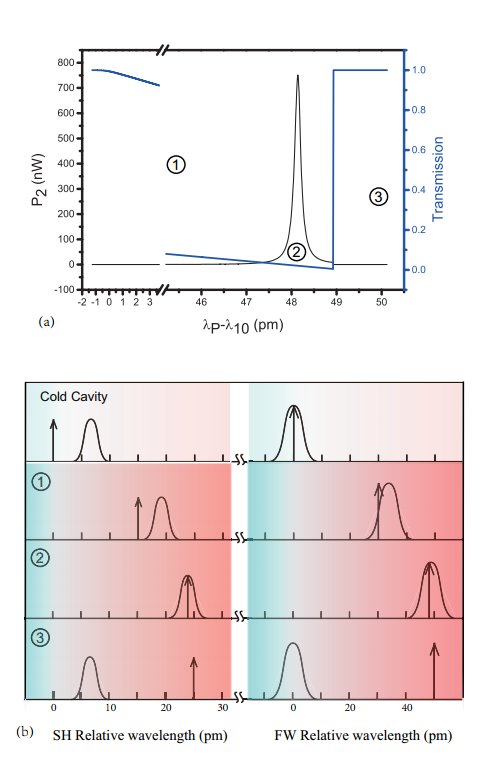
\includegraphics[width=13cm]{try_ed2}
%\caption{\textbf{Third order nonlinearity assisted double resonance. a,} The output SH power (left ordinate, black) and the FW transmission (right ordinate, blue) versus detuning in wavelength between the pump and FW. The numbers in circle indicate three different states corresponding to the schematics with the same number in panel b. \textbf{b,} Schematics of the process to achieve double resonance. The right part is the wavelength relative to the FW wavelength in cold cavity and the left part is the wavelength relative to half of the FW wavelength in cold cavity. Note that the scale of the right part is twice of that on the left. The arrows represent the pump wavelength on the right and half of the pump wavelength on the left. The Lorentz line shapes represent the FW and the SH cavity mode on the right and the left respectively. The top schematics illustrates the relative position of the pump and the cavity mode when the input power is too small to introduce obvious third order nonlinear effects while the lower ones show the position information of the corresponding states in panel a.}

\end{figure}
\begin{figure}
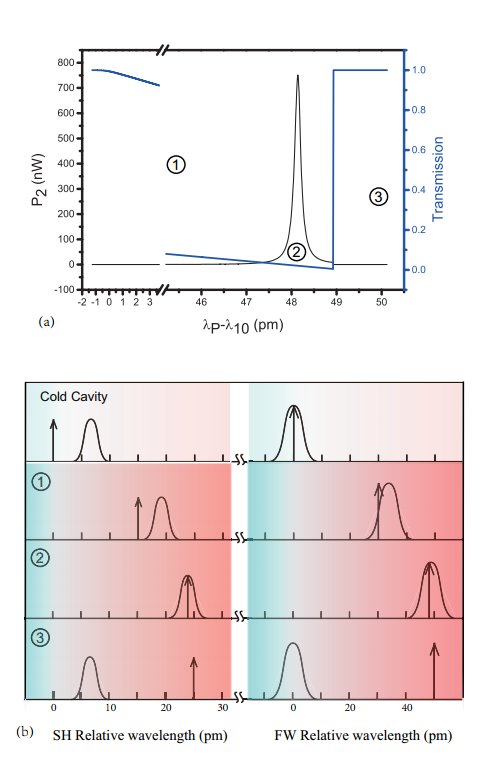
\includegraphics[width=0cm]{try_ed2}
\caption{\textbf{Third order nonlinearity assisted double resonance. a,} The output SH power (left ordinate, black) and the FW transmission (right ordinate, blue) versus detuning in wavelength between the pump and FW. The numbers in circle indicate three different states corresponding to the schematics with the same number in panel b. \textbf{b,} Schematics of the process to achieve double resonance. The right part is the wavelength relative to the FW wavelength in cold cavity and the left part is the wavelength relative to half of the FW wavelength in cold cavity. Note that the scale of the right part is twice of that on the left. The arrows represent the pump wavelength on the right and half of the pump wavelength on the left. The Lorentz line shapes represent the FW and the SH cavity mode on the right and the left respectively. The top schematics illustrates the relative position of the pump and the cavity mode when the input power is too small to introduce obvious third order nonlinear effects while the lower ones show the position information of the corresponding states in panel a.}
\label{pic:try_ed2}
\end{figure}

在二氧化硅腔中,热效应对于腔膜的影响是使腔膜产生一个红移,因而如果要增加输入功率,则腔膜红移,导致输入光和腔膜之间的失谐增大,从而由输入光到腔内能量的转化效率变低,另一方面,如果输入光功率不变,而是在蓝失谐一侧缓慢增加波长,则由于失谐逐渐减小,转化效率逐渐增加,耦合进腔的功率变大,从而使得腔膜再次红移,最终,当转化效率已经达到最大之后,输入光变到腔膜的红失谐处,导致转化效率降低,腔膜蓝移的更加厉害,最终使得输入光几乎不能耦合进腔中\cite{carmon2004dynamical}。

而如果同时考虑二次谐波腔膜的移动,如图\ref{pic:try_ed2}(b)所示,当腔中能量极小时(cold cavity),输入光与基波共振,但其二倍频不与二次谐波模式共振,此时二次谐波产生效率极低。如果输入光功率足够大,则基波和二次谐波腔膜都会发生红移,但是二次谐波腔膜的移动要比输入光的二倍频移动速度慢,则如果开始时输入光二倍频与二次谐波腔膜是蓝失谐的位置关系,则在某一失谐时,能够满足双共振条件图\ref{pic:try_ed2}(b2),此后,如果波长继续增大,则会从两个腔膜中跳出。此过程对应的二次谐波能量和基波经过腔的透射谱如图\ref{pic:try_ed2}(a)所示。

由上述过程可知,如果输入光功率较小,则即使有腔膜移动,也不足以达到双共振条件,因而产生二次谐波功率极低,当输入光功率达到某一临界值时,恰好能够达到双共振条件,当输入光功率继续增大,则在基波达到共振前二次谐波就达到了共振,此时对于实验来说最为稳定,但由于基波未达到共振,虽然输入功率增加了,总体而言产生二次谐波的功率并没有显著变化,该过程如图\ref{pic:P2change_ed2_ai}(a)所示。

转化效率随耦合系数$K$的变化如图\ref{pic:P2change_ed2_ai}(b)所示,在临界耦合的时候转化效率达到最高。不同波长对应的临界功率与色散曲线有关图\ref{pic:P2change_ed2_ai}(c),但一般来说,转化效率与临界功率成正比,这与二次谐波的二阶功率关系是相适应的,同时可以看到,同一个临界功率下,球越大,转化效率会越低,可能是由于球大了之后场比较弥散且更靠近体内,因而表面和体的非线性效应都会有所下降,如图\ref{pic:P2change_ed2_ai}(d)。
\begin{figure}
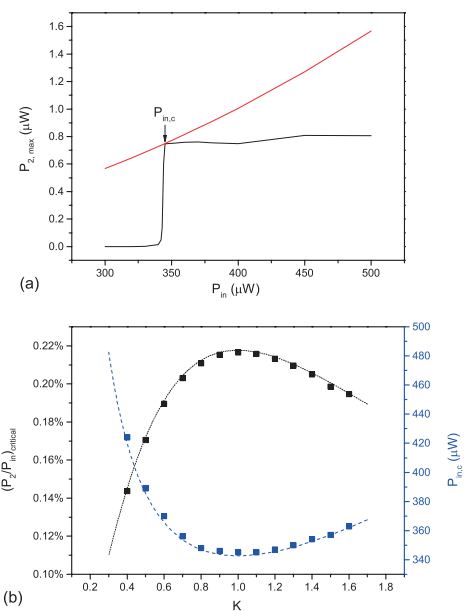
\includegraphics[width=14cm]{P2change_ed2_ai}
\caption{\textbf{Maximum output SH power and efficiency. a,} The maximum output SH power versus input power. The red line is the ideal output SH power by setting the off-resonance coefficient to one. The black line represents the maximum output SH power considering all the possible detuning (corresponds to state 2 in Fig. 2a). \textbf{b, } The conversion efficiency at the critical input power (left ordinate, black) and the critical input power (right ordinate, blue) as a function of coupling coefficient K. The dashed lines are results of the analytical expression and the symbols are calculated numerically with nonlinear coupled-mode equations. \textbf{c-d, } The influence of different diameters of microsphere and various polar order $l$. \textbf{c, }The critical input power versus the FW wavelength. The symbols represents a pair of FW and SH modes with $l_2=2l_1$.  \textbf{d, }The critical conversion efficiency as a function of different critical input power. The symbols are the same with those in panel c and the dashed lines are only guides for the eye. }
\label{pic:P2change_ed2_ai}
\end{figure}

\subsection{实验}
\subsubsection{实验设计}

从原理上考虑实验设计非常简单,只需要将泵浦光有效地耦合进腔,再通过合适的方式探测产生的二次谐波即可,不论是表面还是体多极二次非线性,都是腔内在的性质,不直接依赖于输入输出关系。\cite{carmon2007visible}中的三次谐波产生就只用了最简单的光纤锥耦合的方法,并用CCD摄像头收集产生的绿光。对于本实验来说,将泵浦光耦合进入腔是较为简单的,但是由于信号光的光强非常弱,用一般的CCD无法较好的采集,而如果只用一跟通讯波段的泵浦光纤收集,由于本身与二次谐波模式耦合较弱,再加上二次谐波沿该光纤传播损耗极大,所以不利于收集到较弱的信号光。我们认为,这也是之前的实验当中几乎没有人看到过二次谐波的原因。

为了解决信号光收集问题,选用了双光纤结构,一根是通信波段,用于将泵浦光耦合入腔,另一根在二次谐波波段,专门用于收集二次谐波,并将收集到的二次谐波送入EMCCD中进行光谱分析。

如果仅使用这种实验设计,就完全与\ref{sec:2Resonance}中的理论分析一致,这将会导致二次谐波输出功率随着泵浦光功率呈一个阶跃式的变化,无法验证二次谐波功率与输入功率呈平方关系的特性。因而,在基础实验设计之上,再使用一路控制光源,专门用于调控腔的热效应及Kerr效应,使得达到双共振条件时的腔内泵浦光光强可以在较大范围内变化。

\begin{figure}
\centering
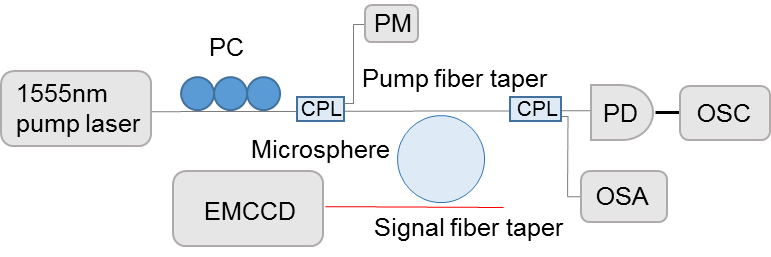
\includegraphics[width=16cm ]{ExpSetup.png}
\caption{实验设计示意图}
\label{pic:ExpSetup}
\end{figure}

如图\ref{pic:ExpSetup}所示,泵浦光在1555nm附近,由于泵浦光需要较强的功率,故用EDFA(掺铒光纤功率放大器)进行功率放大后,经过PC(偏振控制器)调节偏振后,输入耦合光纤锥中。控制光在1550nm附近,由另一台激光器产生,经过PC,并通过CPL(耦合器)与泵浦光合束输入耦合光纤锥中。

经过微腔之后的透射光中依然含有泵浦光和控制光,首先通过CPL分出一部分光进入OSA(光谱仪)中检测通讯波段光谱和拉曼等信号,再经过Y型OBP(光学带通滤波器),通过分波长方法,将泵浦光和控制光分开,并分别输入PD(光探测器)将光信号转化为电信号最后输入OSC(示波器)进行监测。

二次谐波这一路光信号由二次谐波波段的光纤锥进行收集,并送入EMCCD(电子放大电荷耦合器件)中进行光谱探测。

\subsubsection{微球腔的制备}

装置照片,制备步骤,成品照片,Q值,Transmission谱,半径,选取半径值的原因

\subsubsection{双光纤的制备与操控}

拉光纤装置照片,步骤,成品照片,透过率,操控光纤耦合方法,耦合球腔照片



\subsubsection{二次谐波和二次合频信号的产生}

\begin{figure}
\centering
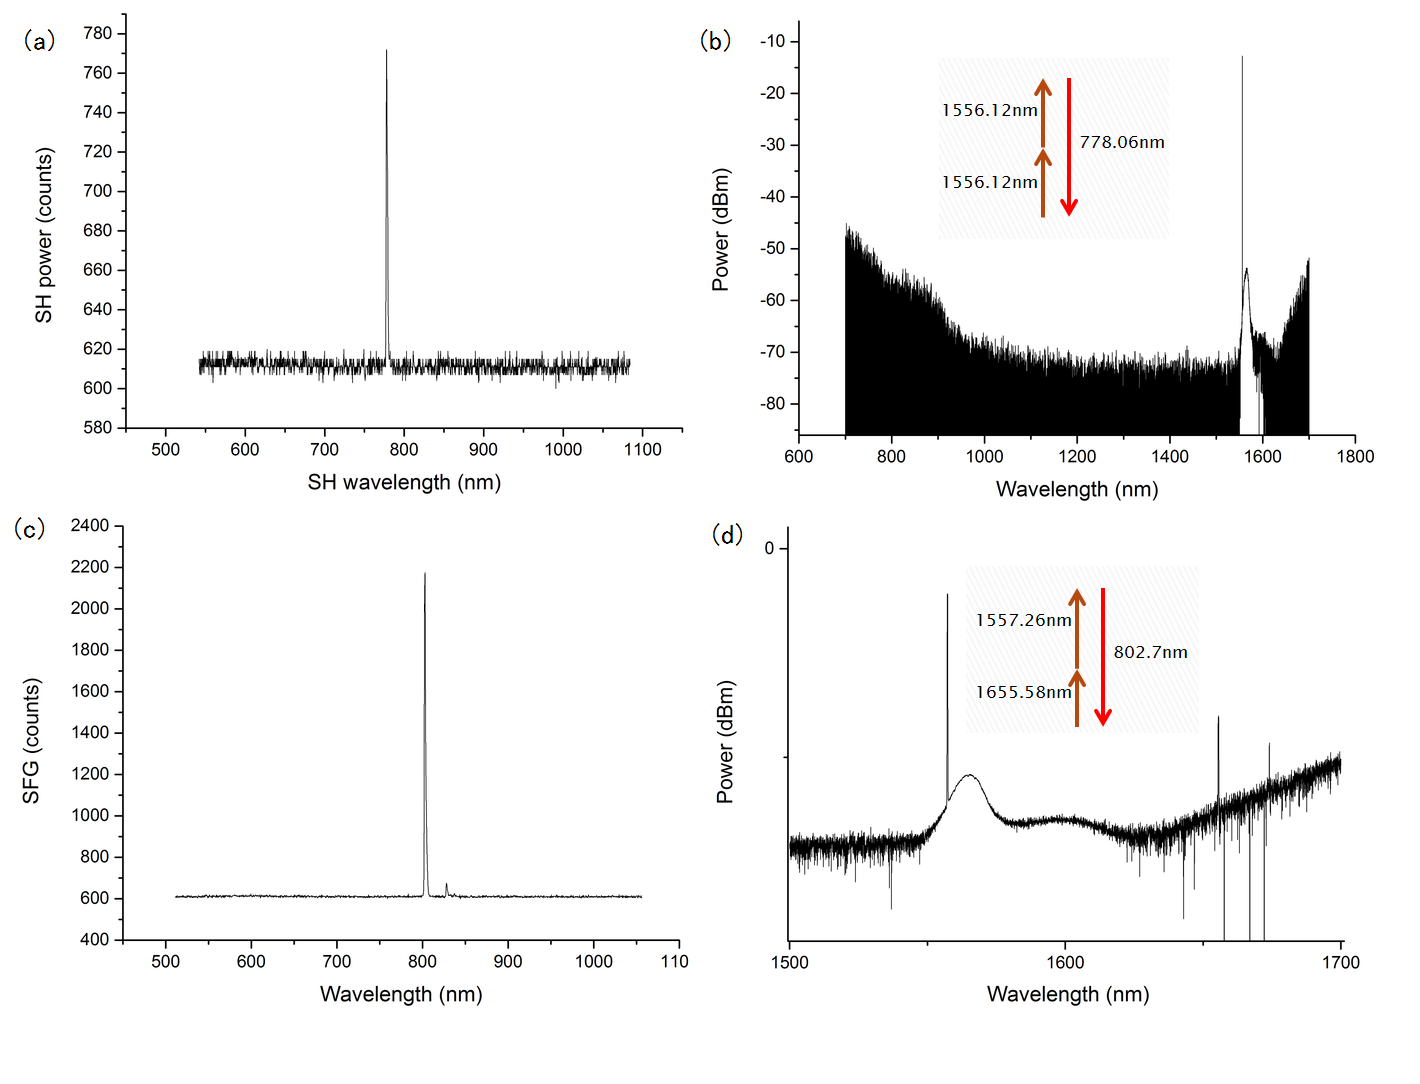
\includegraphics[width=14cm ]{Spectrum.png}
\caption{光谱图。(a)二次谐波信号光谱图。(b)与二次谐波信号对应的泵浦光光谱图,插图为光子能量转换关系说明。(c)二次合频信号光谱图。(d)与二次合频信号对应的泵浦光光谱图,插图为光子能量转换关系说明,两个通讯波段光子分别来自于光谱图上较高的两根线。}
\label{pic:Spectrum}
\end{figure}

为了体现更清晰的物理过程,实验第一步先关闭控制光,在产生二次谐波时输入腔的功率约为25mW。光谱图如图\ref{pic:Spectrum}所示。

\subsubsection{功率依赖关系}

\begin{figure}
\centering
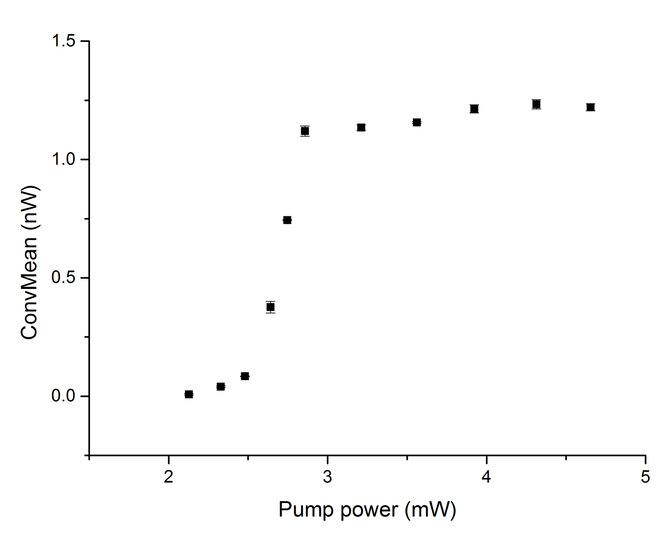
\includegraphics[width=14cm ]{SimpPWDP.png}
\caption{只有泵浦光条件下的二次谐波功率-泵浦光功率依赖关系}
\label{pic:SimpPWDP}
\end{figure}

在只有泵浦光时,由于\ref{sec:2Resonance}中理论分析部分的机理,导致一个几乎为阶跃形式的二次谐波功率-泵浦光功率依赖关系,实验当中测得的曲线如图\ref{pic:SimpPWDP},可以看到这个趋势与图\ref{pic:P2change_ed2_ai}(a)所示几乎一致。






\newpage
\bibliography{ref}
\end{document}




